\documentclass[aspectratio=169]{beamer}
\useoutertheme[progressbar=frametitle]{metropolis}
\useinnertheme{metropolis}
\definecolor{nabgray}{rgb}{0.6,0.59,0.61}
\usecolortheme[named=nabgray]{structure}
\usepackage{tikz}
\usepackage{hyperref}
\usetikzlibrary{mindmap,backgrounds}
\usepackage[utf8]{inputenc}
\usepackage[spanish]{babel}
\usepackage{fontspec}
\usepackage{soul}
\setmonofont{JetBrains Mono}
\setmainfont{Roboto}
\setsansfont{Roboto}

\usepackage{smartdiagram}
\usepackage{qtree}
\usepackage{verbatim}
\usepackage{svg}
\usepackage{graphicx}
\usepackage{color}
\definecolor{lightgray}{rgb}{0.95, 0.95, 0.95}
\definecolor{darkgray}{rgb}{0.4, 0.4, 0.4}
\definecolor{ocherCode}{rgb}{1, 0.5, 0} % #FF7F00 -> rgb(239, 169, 0)
\definecolor{blueCode}{rgb}{0, 0, 0.93} % #0000EE -> rgb(0, 0, 238)
\definecolor{greenCode}{rgb}{0, 0.6, 0} % #009900 -> rgb(0, 153, 0)

\usepackage{upquote}
\usepackage{listings}


\lstset{language=java,
    otherkeywords={var,record},
    % Basic design
    backgroundcolor=\color{lightgray},
    basicstyle={\small\ttfamily},
    frame=l,
    keywordstyle=\footnotesize\color{blue},
    escapeinside={<@}{@>},
    breaklines=true,
    % Line numbers
    xleftmargin={0.75cm},
    numbers=left,
    stepnumber=1,
    firstnumber=1,
    numberfirstline=true
    % Code design
    identifierstyle=\color{black},
    keywordstyle=\color{ocherCode}\bfseries,
    ndkeywordstyle=\color{greenCode}\bfseries,
    stringstyle=\color{ocherCode}\ttfamily,
    commentstyle=\color{darkgray}\ttfamily,
    tabsize=2,
    showtabs=true,
    showspaces=false,
    showstringspaces=false,
    extendedchars=true,
    breaklines=true
}

\lstdefinelanguage{bash}{
    basicstyle=\ttfamily,
    showstringspaces=false,
    commentstyle=\color{red},
    keywordstyle=\color{blue},
    numbers=right,
    xleftmargin={0.25cm}
}
\lstdefinelanguage{Kotlin}{
	comment=[l]{//},
	commentstyle={\color{gray}\ttfamily},
	emph={delegate, filter, first, firstOrNull, forEach, lazy, map, mapNotNull, println, return@},
	emphstyle={\color{purple}},
	identifierstyle=\color{black},
	keywords={abstract, actual, as, as?, break, by, class, companion, continue, data, do, dynamic, else, enum, expect, false, final, for, fun, get, if, import, in, interface, internal, is, null, object, override, package, private, public, return, set, super, suspend, this, throw, true, try, typealias, val, var, vararg, when, where, while},
	keywordstyle={\color{blueCode}\bfseries},
	morecomment=[s]{/*}{*/},
	morestring=[b]",
	morestring=[s]{"""*}{*"""},
	ndkeywords={@Inject, @Deprecated, @JvmField, @JvmName, @JvmOverloads, @JvmStatic, @JvmSynthetic, Array, Byte, Double, Float, Int, Integer, Iterable, Long, Runnable, Short, String},
	ndkeywordstyle={\color{orange}\bfseries},
	sensitive=true,
	stringstyle={\color{olive}\ttfamily},
}


\usebackgroundtemplate
{
    
\includegraphics[width=\paperwidth]{Images/fondo}%
}



\title{Introducción a Kotlin para desarrolladores Java }
\author{Víctor Orozco}
\institute{@tuxtor}
\date{\today}

\begin{document}
{
    \usebackgroundtemplate{
\includegraphics[width=\paperwidth]{Images/portada}}
    \setbeamercolor{frametitle}{fg=red}
    \usebeamercolor[fg]{normal text}
    \frame{\titlepage}
}

\begin{frame}
    \tableofcontents
\end{frame}

{
    \usebackgroundtemplate{
\includegraphics[width=\paperwidth]{Images/separador}}
    \setbeamercolor{normal text}{fg=white}
    \setbeamercolor{frametitle}{fg=red}
    \usebeamercolor[fg]{normal text}
    \section{Contexto}
}


\begin{frame}[fragile]{¿Java?}
\begin{columns}
    \begin{column}{0.5\textwidth}
        \begin{itemize}
            \item Lenguaje (Java 14)
            \item OpenJDK (Java Virtual Machine)
            \item Bibliotecas/API (Java Classpath)
        \end{itemize}
    \end{column}
    \begin{column}{0.5\textwidth}  %%<--- here
        \begin{figure}
            \centering
            
\includegraphics[width=0.4\linewidth]{Images/java}
        \end{figure}
    \end{column}
\end{columns}



El conjunto de los 3 es la plataforma Java(TM) pero pueden usarse de forma independiente
\end{frame}

\begin{frame}[fragile]{Java en Android}

    \begin{columns}
        \begin{column}{0.5\textwidth}
            \begin{itemize}
                \item Lenguaje (Java 7 con algunas cosas de 8)
                \item ART/Dalvik
                \item Bibliotecas/API (Java+Google Classpath)
            \end{itemize}
        \end{column}
        \begin{column}{0.5\textwidth}  %%<--- here
            \begin{figure}
                \centering
                
\includegraphics[width=0.4\linewidth]{Images/java}
            \end{figure}
        \end{column}
    \end{columns}


\end{frame}


\begin{frame}{Java - Java como JVM}

		\begin{figure}
			\centering
			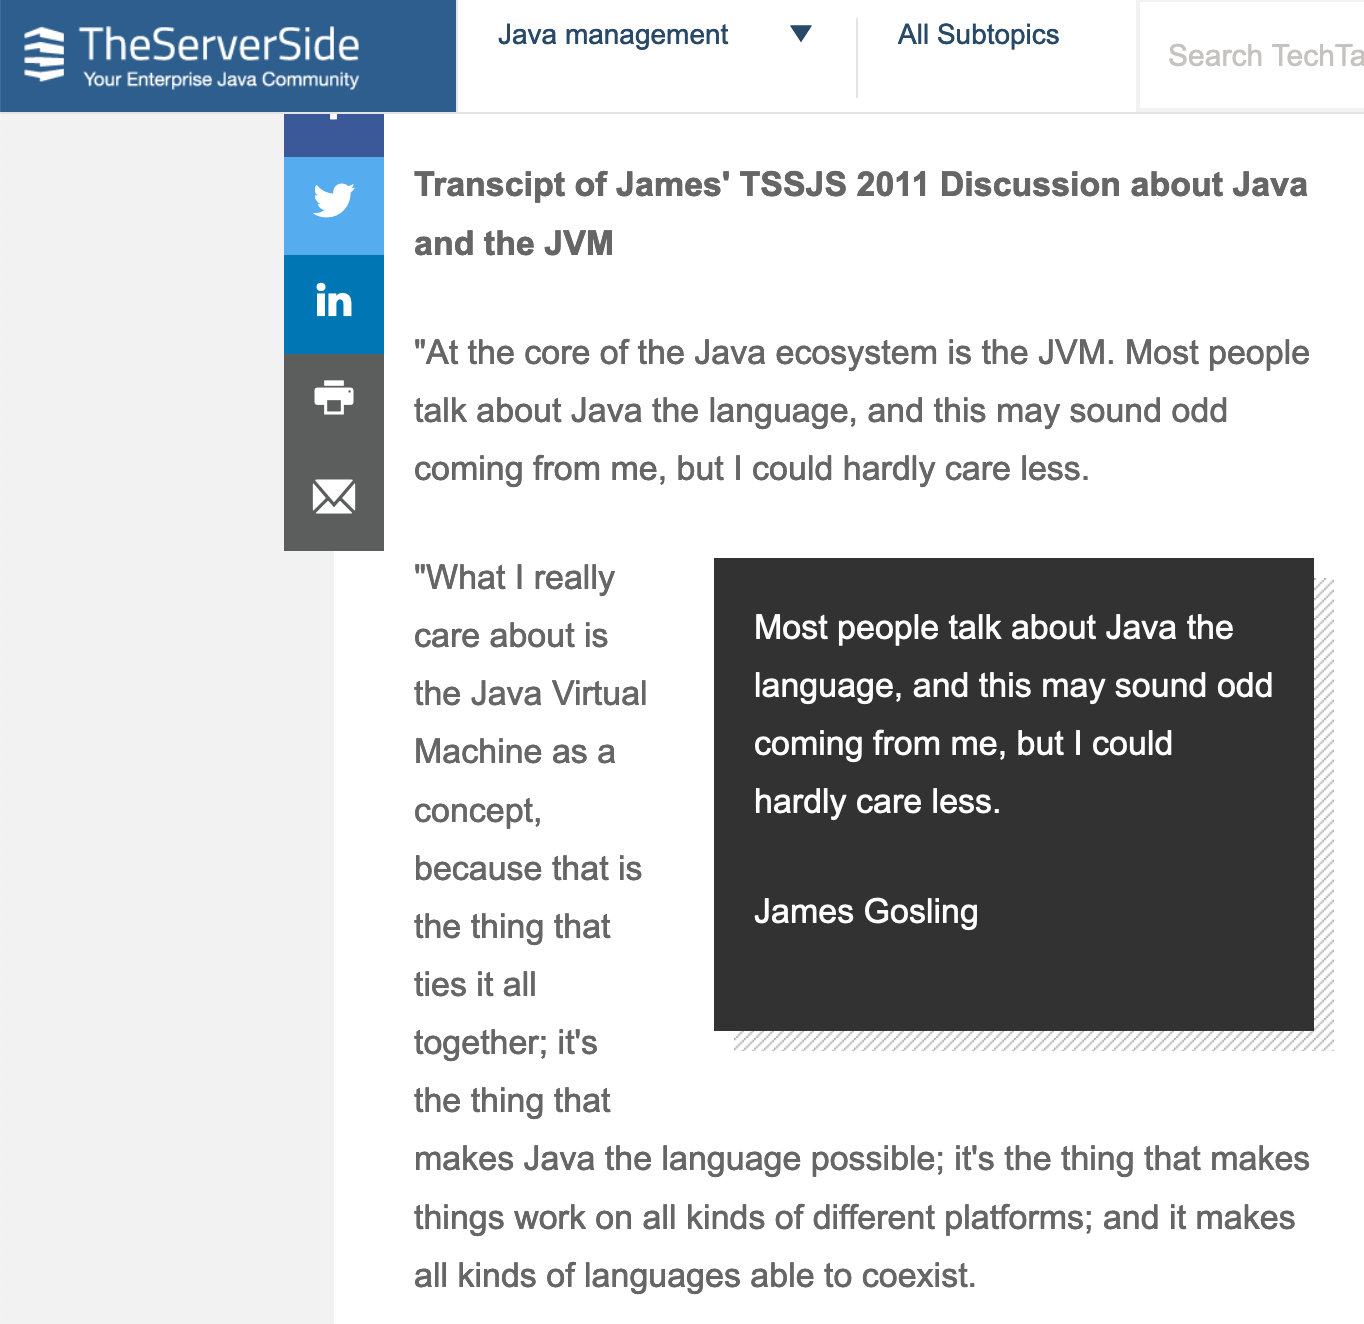
\includegraphics[width=0.7\linewidth]{Images/gossling}
		\end{figure}
\end{frame}


\begin{frame}{JVM}

    \begin{figure}
        \centering
        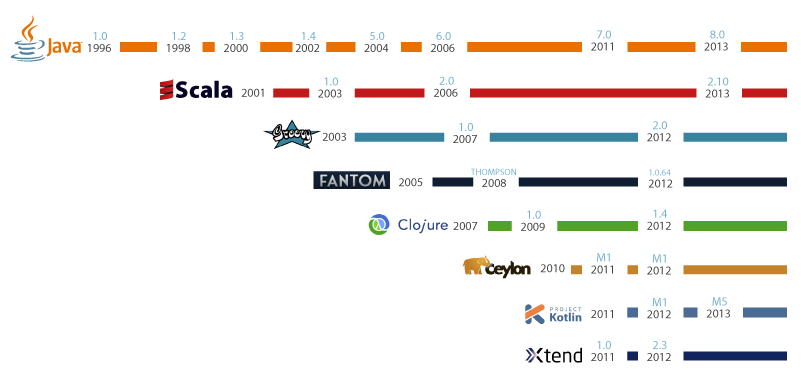
\includegraphics[width=\linewidth]{Images/jvm-languages}
    \end{figure}
\end{frame}

\begin{frame}[fragile]{Kotlin}
    \begin{columns}
        \begin{column}{0.5\textwidth}
            \begin{itemize}
                \item Lenguaje (Kotlin)
                \item OpenJDK (Java Virtual Machine)
                \item Bibliotecas/API (Java Classpath)
                \item kotlin-stdlib
            \end{itemize}
        \end{column}
        \begin{column}{0.5\textwidth}  %%<--- here
            \begin{figure}
                \centering
                
\includegraphics[width=0.4\linewidth]{Images/kotlin}
            \end{figure}
        \end{column}
    \end{columns}
\end{frame}

\begin{frame}[fragile]{Kotlin en Android}
    \begin{columns}
        \begin{column}{0.5\textwidth}
            \begin{itemize}
                \item Lenguaje (Kotlin)
                \item ART/Dalvik
                \item Bibliotecas/API (Java+Google Classpath)
                \item kotlin-stdlib
            \end{itemize}
        \end{column}
        \begin{column}{0.5\textwidth}  %%<--- here
            \begin{figure}
                \centering
                
\includegraphics[width=0.4\linewidth]{Images/kotlin}
            \end{figure}
        \end{column}
    \end{columns}
\end{frame}

\begin{frame}[fragile]{Kotlin en JS}

    \begin{columns}
        \begin{column}{0.5\textwidth}
            \begin{itemize}
                \item Lenguaje (Kotlin)
                \item V8/SpiderMonkey
                \item Bibliotecas/API (ECMA 6 + Web)
                \item kotlin-stdlib
            \end{itemize}
        \end{column}
        \begin{column}{0.5\textwidth}  %%<--- here
            \begin{figure}
                \centering
                
\includegraphics[width=0.4\linewidth]{Images/kotlin}
            \end{figure}
        \end{column}
    \end{columns}
\end{frame}

\begin{frame}[fragile]{Kotlin Nativo}
    \begin{columns}
        \begin{column}{0.5\textwidth}
            \begin{itemize}
                \item Lenguaje (Kotlin)
                \item LLVM
                \item GLibc (Linux)
                \item kotlin-stdlib
            \end{itemize}
        \end{column}
        \begin{column}{0.5\textwidth}  %%<--- here
            \begin{figure}
                \centering
                
\includegraphics[width=0.4\linewidth]{Images/kotlin}
            \end{figure}
        \end{column}
    \end{columns}

\end{frame}

\begin{frame}[fragile]{Kotlin Nativo/GraalVM}
    \begin{columns}
        \begin{column}{0.5\textwidth}
            \begin{itemize}
                \item Lenguaje (Kotlin)
                \item GraalVM Native
                \item Bibliotecas/API (Java Classpath)
                \item kotlin-stdlib
            \end{itemize}
        \end{column}
        \begin{column}{0.5\textwidth}  %%<--- here
            \begin{figure}
                \centering
                
\includegraphics[width=0.4\linewidth]{Images/kotlin}
            \end{figure}
        \end{column}
    \end{columns}
\end{frame}



\begin{frame}[fragile]{Kotlin como lenguaje}
    \begin{columns}
        \begin{column}{0.5\textwidth}
            \begin{itemize}
                \item Típado estático con inferencia de tipos
                \item OOP y funcional
                \item Funciones son ciudadanos de primer nivel
                \item Interoperable con Java
                \item Compilador genera Bytecode nivel Java 6 (Android)
            \end{itemize}
        \end{column}
        \begin{column}{0.5\textwidth}  %%<--- here
            \begin{figure}
                \centering
                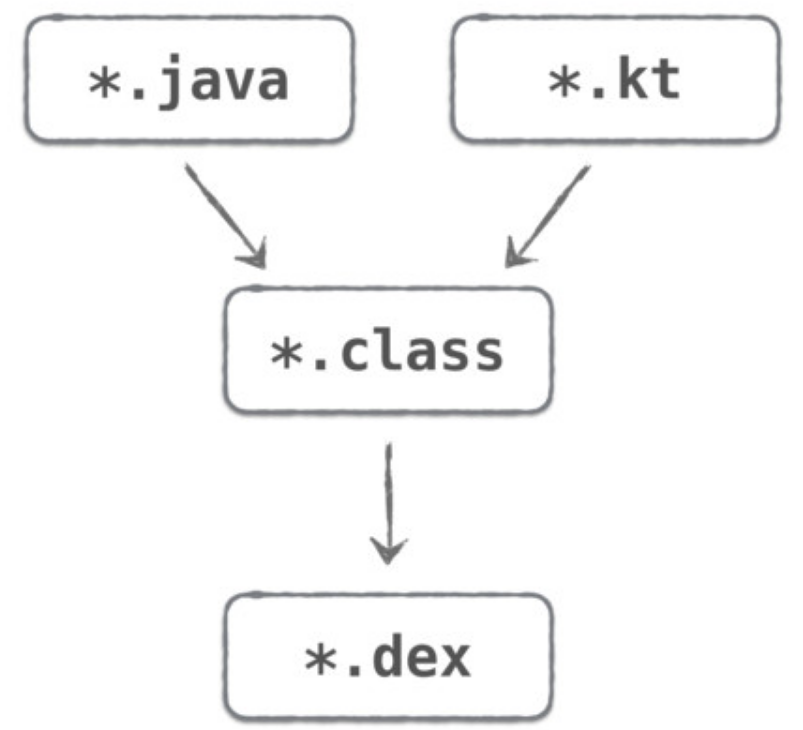
\includegraphics[width=0.8\linewidth]{Images/compile}
            \end{figure}
        \end{column}
    \end{columns}

\end{frame}

{
    \usebackgroundtemplate{
\includegraphics[width=\paperwidth]{Images/separador}}
    \setbeamercolor{normal text}{fg=white}
    \setbeamercolor{frametitle}{fg=red}
    \usebeamercolor[fg]{normal text}
    \section{Caracteristicas interesantes}
}


\begin{frame}[fragile]{Kotlin - Inferencia de tipos (constantes y variables)}
Similar a lo visto en TypeScript o Swift, promueve la inmutabilidad
\begin{lstlisting}[language=Kotlin]
// Mutable
var answer = 42

// Inmutable
val phrase = "JVM Rocks!"

// Declaración explicita
val pi : Double = "3.14159"

// Inferencia por retorno
val auto = crearAuto()
\end{lstlisting}

\end{frame}

\begin{frame}[fragile]{Kotlin - Funciones}

Pueden ser \textit{top level, nested y a su vez pueden ser bloques o expresiones}
\begin{lstlisting}[language=Kotlin]
//Bloque
fun sumar(x: Int, y: Int): Int{
    return x + y
}

//One-line - Expresion y default parameter
fun sumar2(x: Int, y: Int = 99) = x + y

//Infix - AKA operador
infix fun Int.sumar3(y: Int) = this + y
...
//Uso
2 sumar3 4
\end{lstlisting}

\end{frame}

\begin{frame}[fragile]{Kotlin - Clases}
Todas las clases heredan de \textit{Any}
\begin{lstlisting}[language=Kotlin]
//Clase
class Automovil: Vehiculo{
    ...
    constructor(conductor:Persona): super(conductor){
        ...
    }
}

//Clase concisa
class Automovil(conductor:Persona): Vehiculo(conductor){
    ...
}
\end{lstlisting}

\end{frame}

\begin{frame}[fragile]{Kotlin - Propiedades y clases}
Combinación del campo y métodos de acceso
\begin{lstlisting}[language=Kotlin]
//Clase
class Automovil: Vehiculo{
    var marca: String
    var modelo: Int = 2020
    var motor: String = ""
        set(value) {
            field = value + "CC"
        }
        get() = field + " extra info"
}
\end{lstlisting}

\end{frame}

\begin{frame}[fragile]{Kotlin - Clases}
Kotlin permite escribir clases y data carriers de forma concisa
\begin{lstlisting}[language=Kotlin]
//Forma corta
class Automovil(val marca: String, val color: String="Rojo")
...
//Data class (metodos universales como equals, hash code, toString)
data class Automovil(val marca: String,
    val color: String="Rojo")
\end{lstlisting}

\end{frame}


\begin{frame}[fragile]{Kotlin - Object AKA Singleton}
Creación de instancias únicas
\begin{lstlisting}[language=Kotlin]
object Automovil: Vehiculo {
    override fun correr(){
        ...
    }
}

//Invocamos comportamiento
Automovil.correr()


//Y lo usamos como objeto
fun iniciarVehiculo(Automovil)
\end{lstlisting}

\end{frame}

\begin{frame}[fragile]{Kotlin - No static keyword}

\begin{lstlisting}[language=Kotlin]
class Automovil {
    companion object {
        fun correr() {
            ...
        }
    }
}

object Automovil {
    override fun correr(){
    ...
    }
}
\end{lstlisting}

\end{frame}


\begin{frame}[fragile]{Kotlin - Extension functions}
Posibilidad de extender funcionalidad en clases existentes
\begin{lstlisting}[language=Kotlin]
fun String.ultimoCar(): Char = this.get(this.lenght - 1)

val frase: Char = "Yo amo la JVM".ultimoCar()
\end{lstlisting}

\end{frame}


\begin{frame}[fragile]{Kotlin - Verificación de nulos}
En Kotlin la verificación de nulos y declaración de variables "abiertas" es explicita
\begin{lstlisting}[language=Kotlin]
val talvez: String? = ...

talvez.length //Error de compilacion
talvez?.length

fun forzarNull(s: String?) {
    println(s!!.length)
}

\end{lstlisting}

\end{frame}

\begin{frame}[fragile]{Kotlin - Smart Cast y Pattern Matching}
El casting se da automático en ciertos bloques y expresiones
\begin{lstlisting}[language=Kotlin]
val auto1: Vehiculo = ...

if (auto1 is Automovil){
    auto1.cosasDeAutos()
}

when (auto1) {
    is Automovil -> auto1.cosasDeAutos()
    is Motocicleta -> auto1.cosasDemotos()
    else -> throw Exception("El vehiculo de los ojos tristes")
}

\end{lstlisting}

\end{frame}


\begin{frame}[fragile]{Kotlin - Collections}
Metodos convenientes y expresiones lambda, por defecto Inmutables
\begin{lstlisting}[language=Kotlin]
//Con expresiones lambda
listOf(1, 2, 3).filter{ i -> i % 2 == 0}

//Con expresiones cortas (predicado)
listOf(1, 2, 3).filter{i % 2 == 0}
\end{lstlisting}
\end{frame}

\begin{frame}{Kotlin - Convenciones}
    \begin{columns}
        \begin{column}{0.5\textwidth}
            \begin{itemize}
                \item Convenciones de nombrado Java
                \item Típos en Uppercase
                \item Metodos y propiedades en lower camelCase
                \item Punto y coma son opcionales
                \item Convención reversa en nombrado de paquetes
                \item Multiples clases por archivo
                \item Los paquetes en código no deben coincidir con nombres de directorios
            \end{itemize}
        \end{column}
        \begin{column}{0.5\textwidth}  %%<--- here
            \begin{figure}
                \centering
                
\includegraphics[width=0.7\linewidth]{Images/semicolon}
            \end{figure}
        \end{column}
    \end{columns}
\end{frame}

{
    \usebackgroundtemplate{
\includegraphics[width=\paperwidth]{Images/separador}}
    \setbeamercolor{normal text}{fg=white}
    \setbeamercolor{frametitle}{fg=red}
    \usebeamercolor[fg]{normal text}
    \section{Demo productiva}
}


\begin{frame}{Eclipse MicroProfile - 1, 2, 3 with Kotlin}
\begin{enumerate}
	\item Maven or Gradle config
	\item MicroProfile dependency and your extras (Jakarta EE, Arquillian, JUnit, . . .)
	\item Maven plugin (maven-compiler-plugin)
	\item Kotlin plugin (kotlin-maven-plugin)
\end{enumerate}
\end{frame}

\begin{frame}[fragile]{Eclipse MicroProfile with Payara 5}
\begin{lstlisting}
<dependency>
    <groupId>org.eclipse.microprofile</groupId>
    <artifactId>microprofile</artifactId>
    <type>pom</type>
    <version>3.2</version>
    <scope>provided</scope>
</dependency>
\end{lstlisting}
\end{frame}


\begin{frame}[fragile]{Kotlin with Maven - Dependency}
\begin{lstlisting}[language=XML]
<dependency>
    <groupId>org.jetbrains.kotlin</groupId>
    <artifactId>kotlin-stdlib-jdk8</artifactId>
    <version>${kotlin.version}</version>
</dependency>
\end{lstlisting}
\end{frame}

\begin{frame}[fragile]{Kotlin with Maven - maven-compiler-plugin}
\begin{lstlisting}[language=xml,
basicstyle=\tiny\ttfamily
]
<execution>
    <id>default-compile</id>
    <phase>none</phase>
</execution>
<execution>
    <id>default-testCompile</id>
    <phase>none</phase>
</execution>
<execution>
    <id>java-compile</id>
    <phase>compile</phase>
    <goals> <goal>compile</goal> </goals>
</execution>
<execution>
    <id>java-test-compile</id>
    <phase>test-compile</phase>
    <goals> <goal>testCompile</goal> </goals>
</execution>
\end{lstlisting}
\end{frame}


\begin{frame}[fragile]{Kotlin with Maven - kotlin-maven-plugin}
\begin{lstlisting}[
basicstyle=\tiny\ttfamily
]
<compilerPlugins>
    <plugin>all-open</plugin>
</compilerPlugins>
...
<option>all-open:annotation=javax.ws.rs.Path</option>
<option>all-open:annotation=javax.enterprise.context.RequestScoped</option>
<option>all-open:annotation=javax.enterprise.context.SessionScoped</option>
<option>all-open:annotation=javax.enterprise.context.ApplicationScoped</option>
<option>all-open:annotation=javax.enterprise.context.Dependent</option>
<option>all-open:annotation=javax.ejb.Singleton</option>
<option>all-open:annotation=javax.ejb.Stateful</option>
<option>all-open:annotation=javax.ejb.Stateless</option>
\end{lstlisting}

Idea general: Agregar todas las anotaciones arquitecturales de JakartaEE (CDI and EJB)
\end{frame}

\begin{frame}{Kotlin + Jakarta EE + MicroProfile  - Demo}

\begin{itemize}
	\item Kotlin 1.4.x
	\item Libraries - SLF4J, Flyway, PostgreSQL
	\item Jakarta EE 8 - EJB, JPA
	\item MicroProfile - CDI, JAX-RS, MicroProfile Config
	\item Testing - Arquillian, JUnit, Payara Embedded
\end{itemize}


\normalsize  \url{https://dzone.com/articles/the-state-of-kotlin-for-jakarta-eemicroprofile-tra}\\
\normalsize  \url{https://github.com/tuxtor/integrum-ee}
\end{frame}

\begin{frame}{Kotlin + Jakarta EE + MicroProfile  - Demo}
\begin{figure}
	\centering
	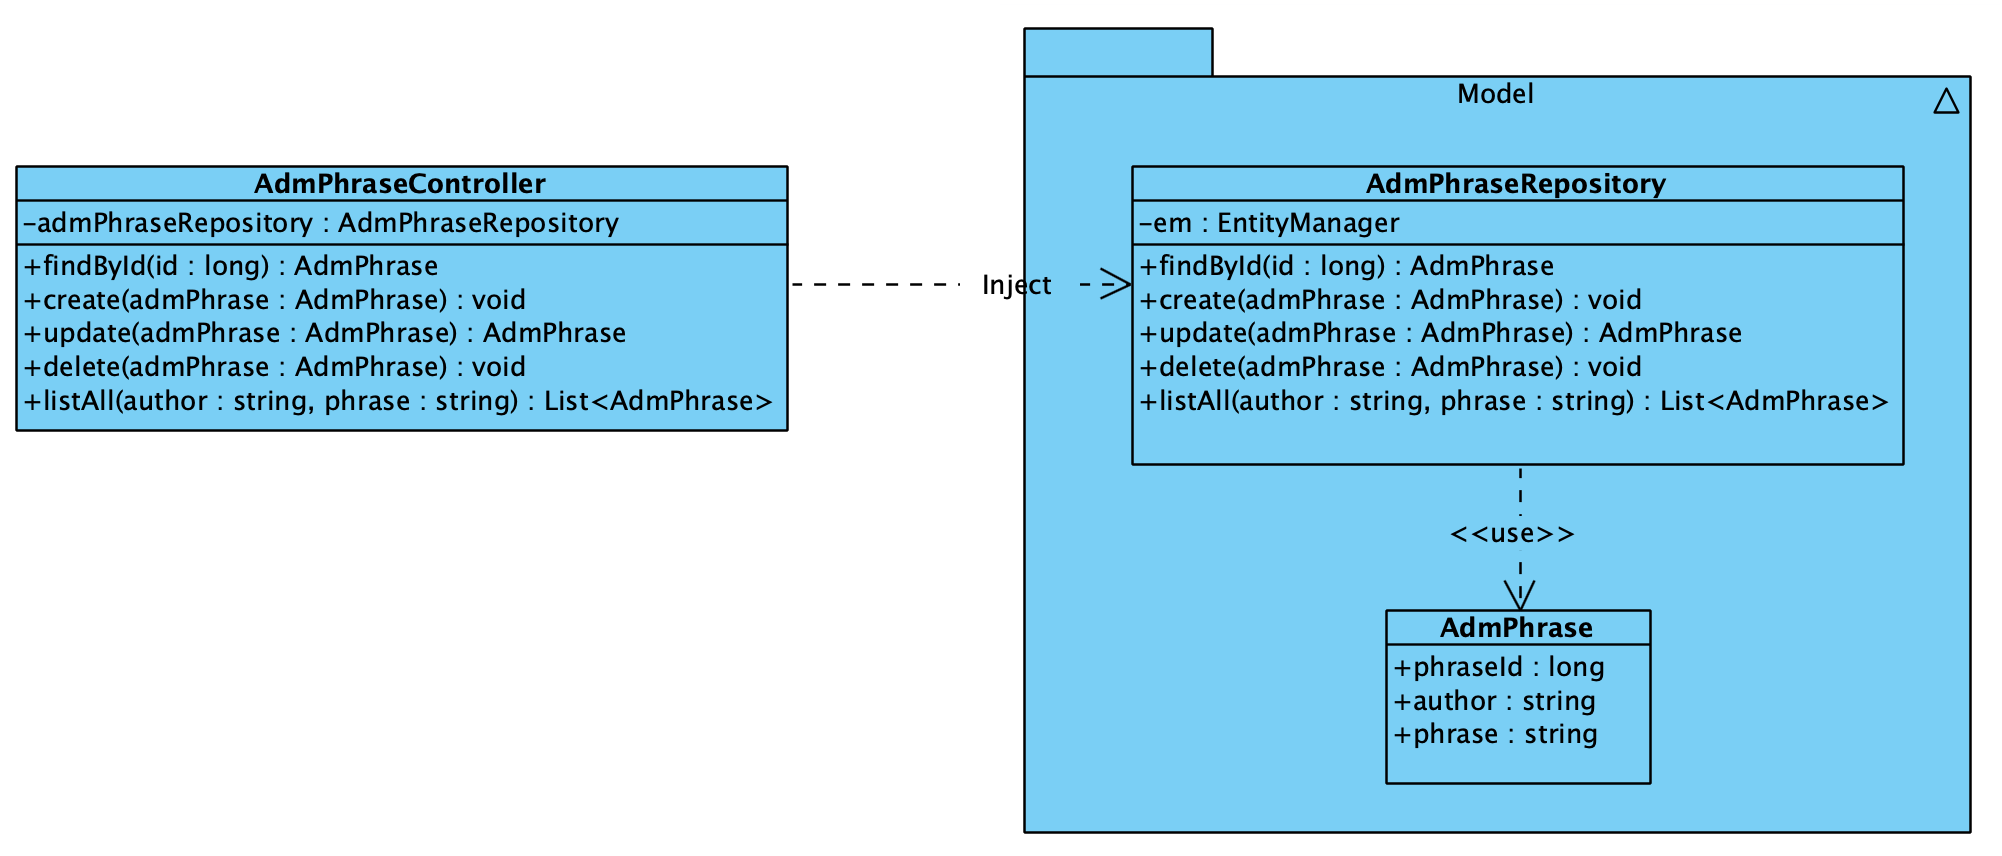
\includegraphics[width=\linewidth]{Images/integrum-ee}
\end{figure}
\end{frame}

\begin{frame}{Kotlin + Jakarta EE + MicroProfile  - Demo}
\begin{figure}
	\centering
	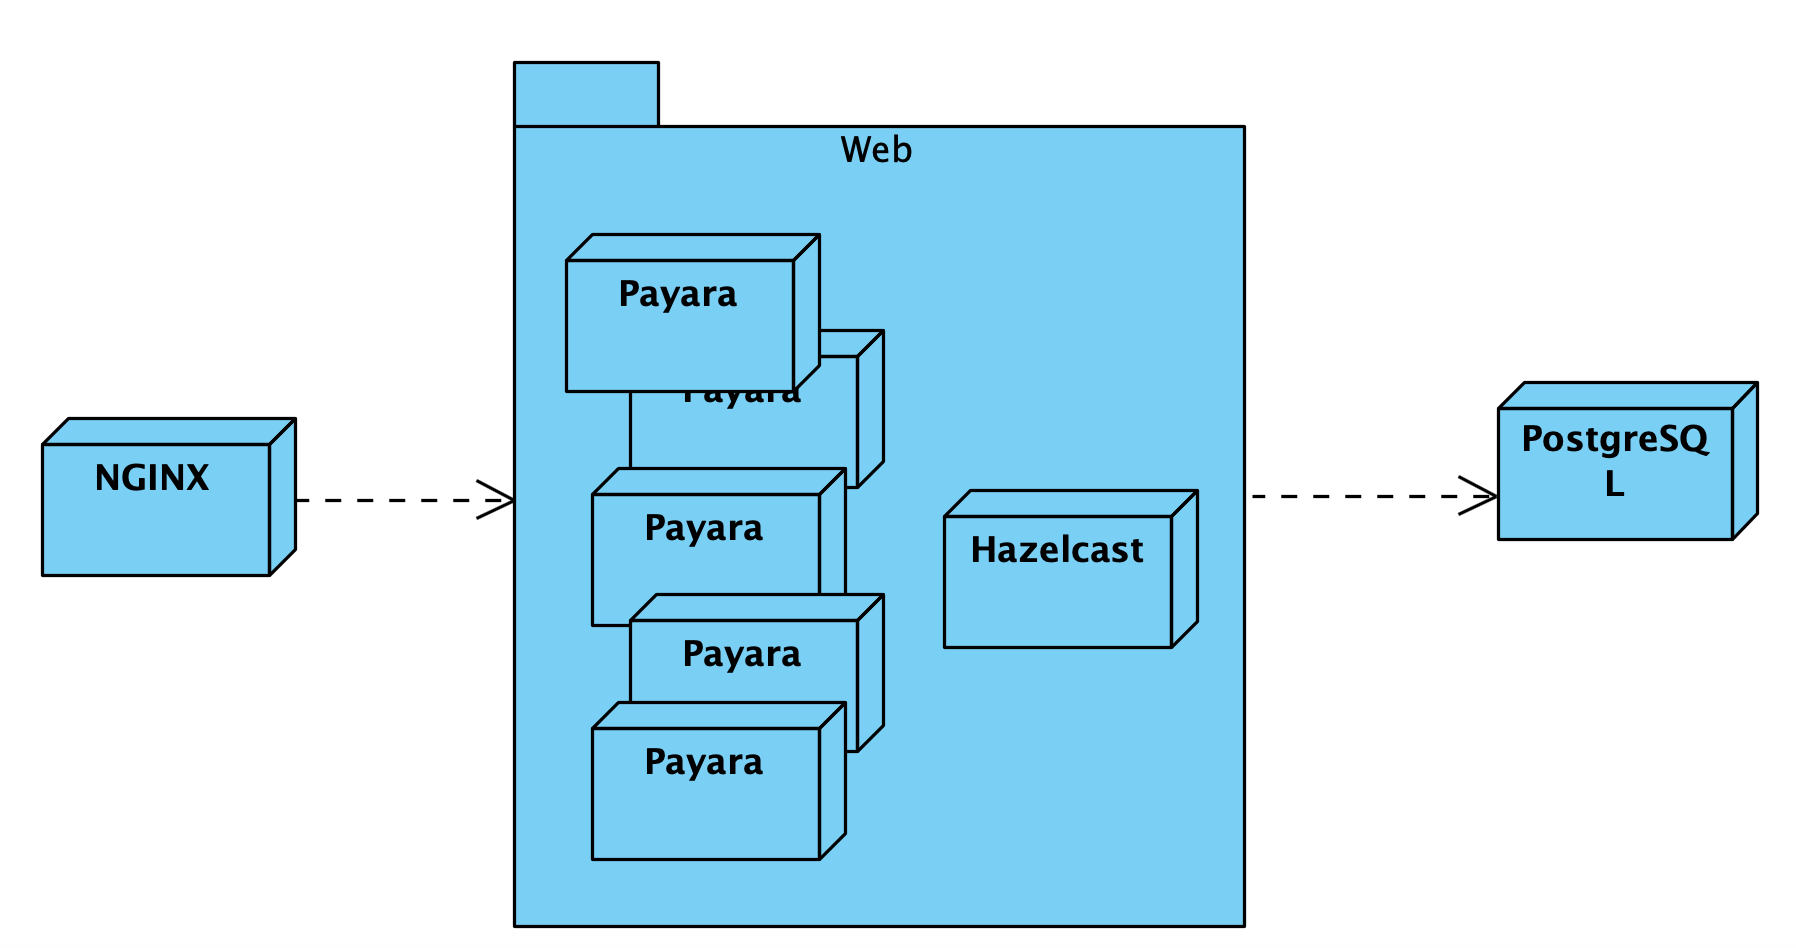
\includegraphics[width=\linewidth]{Images/integrum-deployment}
\end{figure}
\end{frame}


\begin{frame}[fragile]{Kotlin - JPA entity}
\begin{lstlisting}[language=Kotlin]
@Entity
@Table(name = "adm_phrase")
@TableGenerator(...)
data class AdmPhrase(
    @Id
    @GeneratedValue(strategy = GenerationType.TABLE,
        generator = "admPhraseIdGenerator")
    @Column(name = "phrase_id")
    var phraseId:Long? = null,
    var author:String = "",
    var phrase:String = ""
)
\end{lstlisting}
Data Clases, Nullable Types
\end{frame}

\begin{frame}[fragile]{Kotlin - CDI Repository}
\begin{lstlisting}[language=Kotlin]
@RequestScoped
class AdmPhraseRepository {

    @Inject
    private lateinit var em:EntityManager

    ...

}
\end{lstlisting}
Lateinit (nullable type)
\end{frame}

\begin{frame}[fragile]{Kotlin - CDI Repository}
\begin{lstlisting}[language=Kotlin]
fun create(admPhrase:AdmPhrase) = em.persist(admPhrase)

fun update(admPhrase:AdmPhrase) = em.merge(admPhrase)

fun findById(phraseId: Long) =
em.find(AdmPhrase::class.java, phraseId)

fun delete(admPhrase: AdmPhrase) = em.remove(admPhrase)
. . .
\end{lstlisting}
Single expression functions (One line methods)
\end{frame}

\begin{frame}[fragile]{Kotlin - CDI Repository}
\begin{lstlisting}[language=Kotlin]
fun listAll(author: String, phrase: String):
    List<AdmPhrase> {

    val query = """SELECT p FROM AdmPhrase p
    where p.author LIKE :author
    and p.phrase LIKE :phrase
    """

    return em.createQuery(query, AdmPhrase::class.java)
        .setParameter("author", "%$author%")
        .setParameter("phrase", "%$phrase%")
        .resultList
}
\end{lstlisting}
Multiline string
\end{frame}

\begin{frame}[fragile]{Kotlin - JAX-RS Controllers}
\begin{lstlisting}[language=Kotlin, basicstyle=\scriptsize\ttfamily]
@Path("/phrases")
@Produces(MediaType.APPLICATION_JSON)
@Consumes(MediaType.APPLICATION_JSON)
class AdmPhraseController{

    @Inject
    private lateinit var admPhraseRepository: AdmPhraseRepository

    @Inject
    private lateinit var logger: Logger
    ...

}
\end{lstlisting}
\end{frame}

\begin{frame}[fragile]{Kotlin - JAX-RS Controller}
\begin{lstlisting}[language=Kotlin, basicstyle=\scriptsize\ttfamily]

@GET
fun findAll(
@QueryParam("author") @DefaultValue("%") author: String,
@QueryParam("phrase") @DefaultValue("%") phrase: String) =
    admPhraseRepository.listAll(author, phrase)

@GET
@Path("/{id:[0-9][0-9]*}")
fun findById(@PathParam("id") id:Long) =
    admPhraseRepository.findById(id)

@PUT
fun create(phrase: AdmPhrase): Response {
    admPhraseRepository.create(phrase)
    return Response.ok().build()
}
\end{lstlisting}
\end{frame}


\begin{frame}[fragile]{Kotlin - JAX-RS Controller}
Elvis operator as expression
\begin{lstlisting}[language=Kotlin, basicstyle=\scriptsize\ttfamily]
@POST
@Path("/{id:[0-9][0-9]*}")
fun update(@PathParam("id") id: Long?, phrase: AdmPhrase)
    :Response {
    if(id != phrase.phraseId)
        return Response.status(Response.Status.NOT_FOUND).build()

    val updatedEntity = admPhraseRepository.update(phrase)
    return Response.ok(updatedEntity).build()
}

@DELETE
@Path("/{id:[0-9][0-9]*}")
fun delete(@PathParam("id") id: Long): Response {
    val updatedEntity = admPhraseRepository.findById(id) ?:
    return Response.status(Response.Status.NOT_FOUND).build()
    admPhraseRepository.delete(updatedEntity)
    return Response.ok().build()
}
\end{lstlisting}

\end{frame}

\begin{frame}[fragile]{Oracle Cloud}
\begin{lstlisting}[language=XML, basicstyle=\scriptsize\ttfamily]
<groupId>io.fabric8</groupId>
<artifactId>docker-maven-plugin</artifactId>
<version>0.30.0</version>
...
<image>
    <name>iad.ocir.io/tuxtor/microprofile/integrum-ee</name>
    <build>
        <dockerFile>${project.basedir}/Dockerfile</dockerFile >
    </build>
</image>
\end{lstlisting}
\end{frame}

\begin{frame}{Oracle Cloud}
\begin{figure}
	\centering
	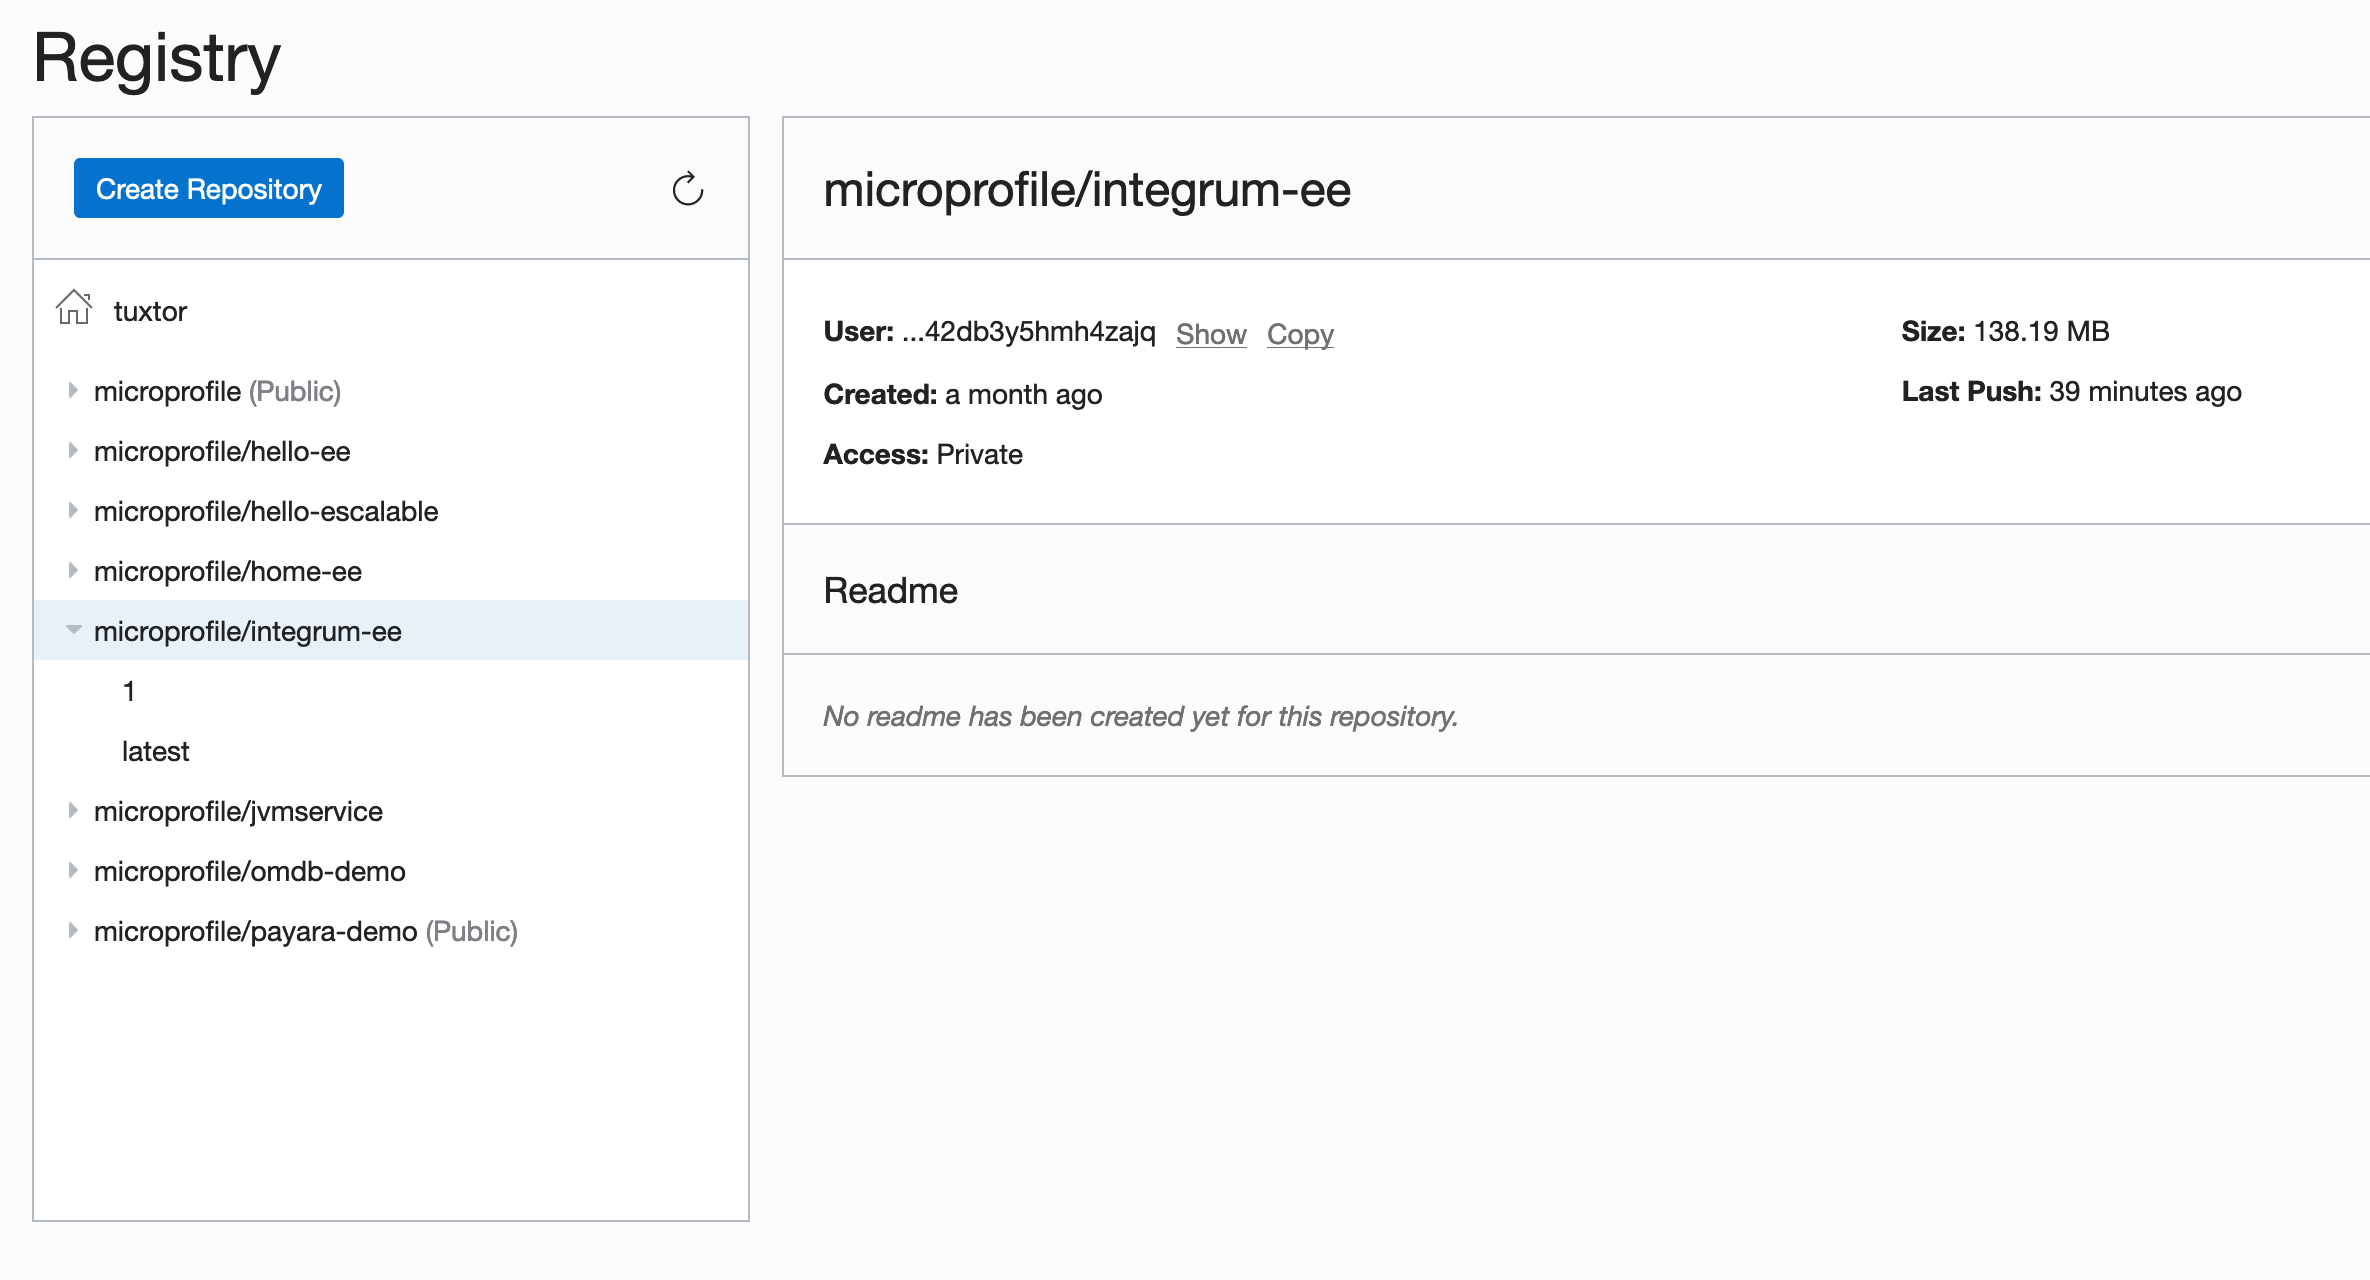
\includegraphics[width=0.95\linewidth]{Images/oc1}
\end{figure}
\end{frame}

\begin{frame}{Oracle Cloud}
\begin{figure}
	\centering
	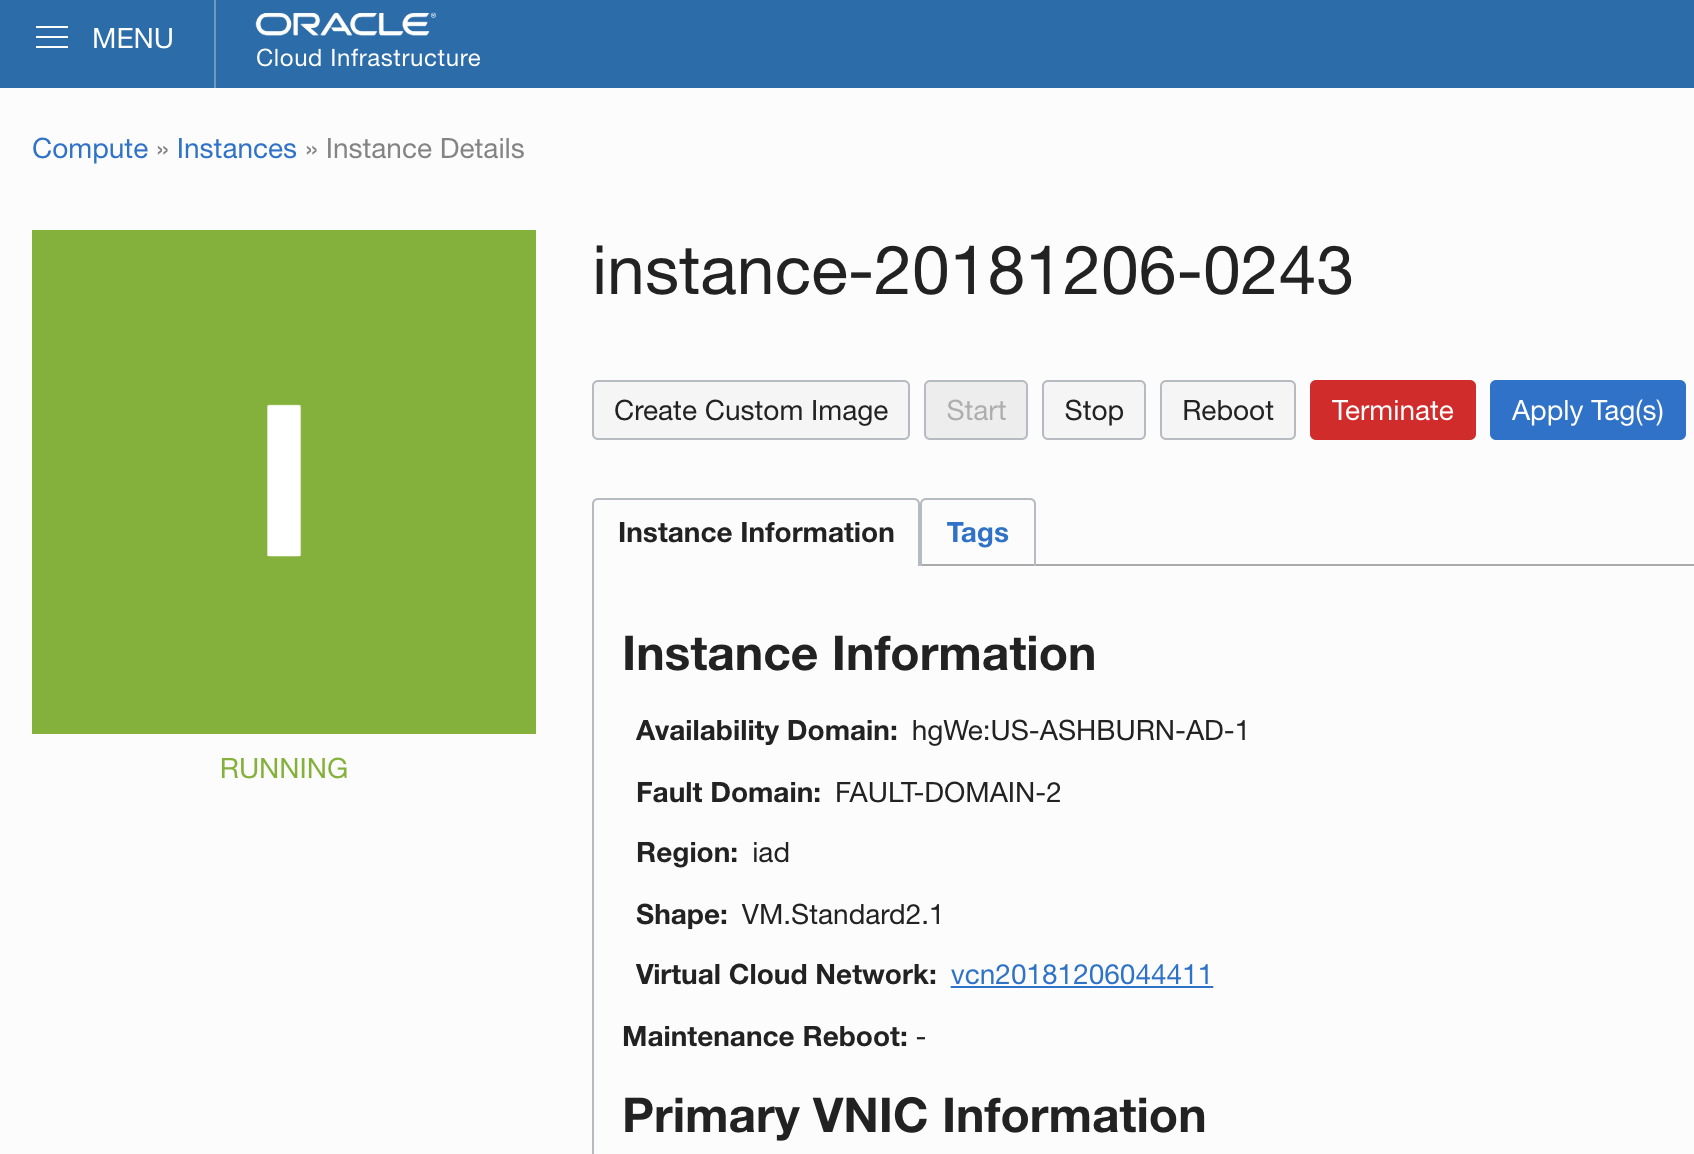
\includegraphics[width=0.95\linewidth]{Images/oc2}
\end{figure}
\end{frame}

\begin{frame}{Oracle Cloud}
\begin{figure}
	\centering
	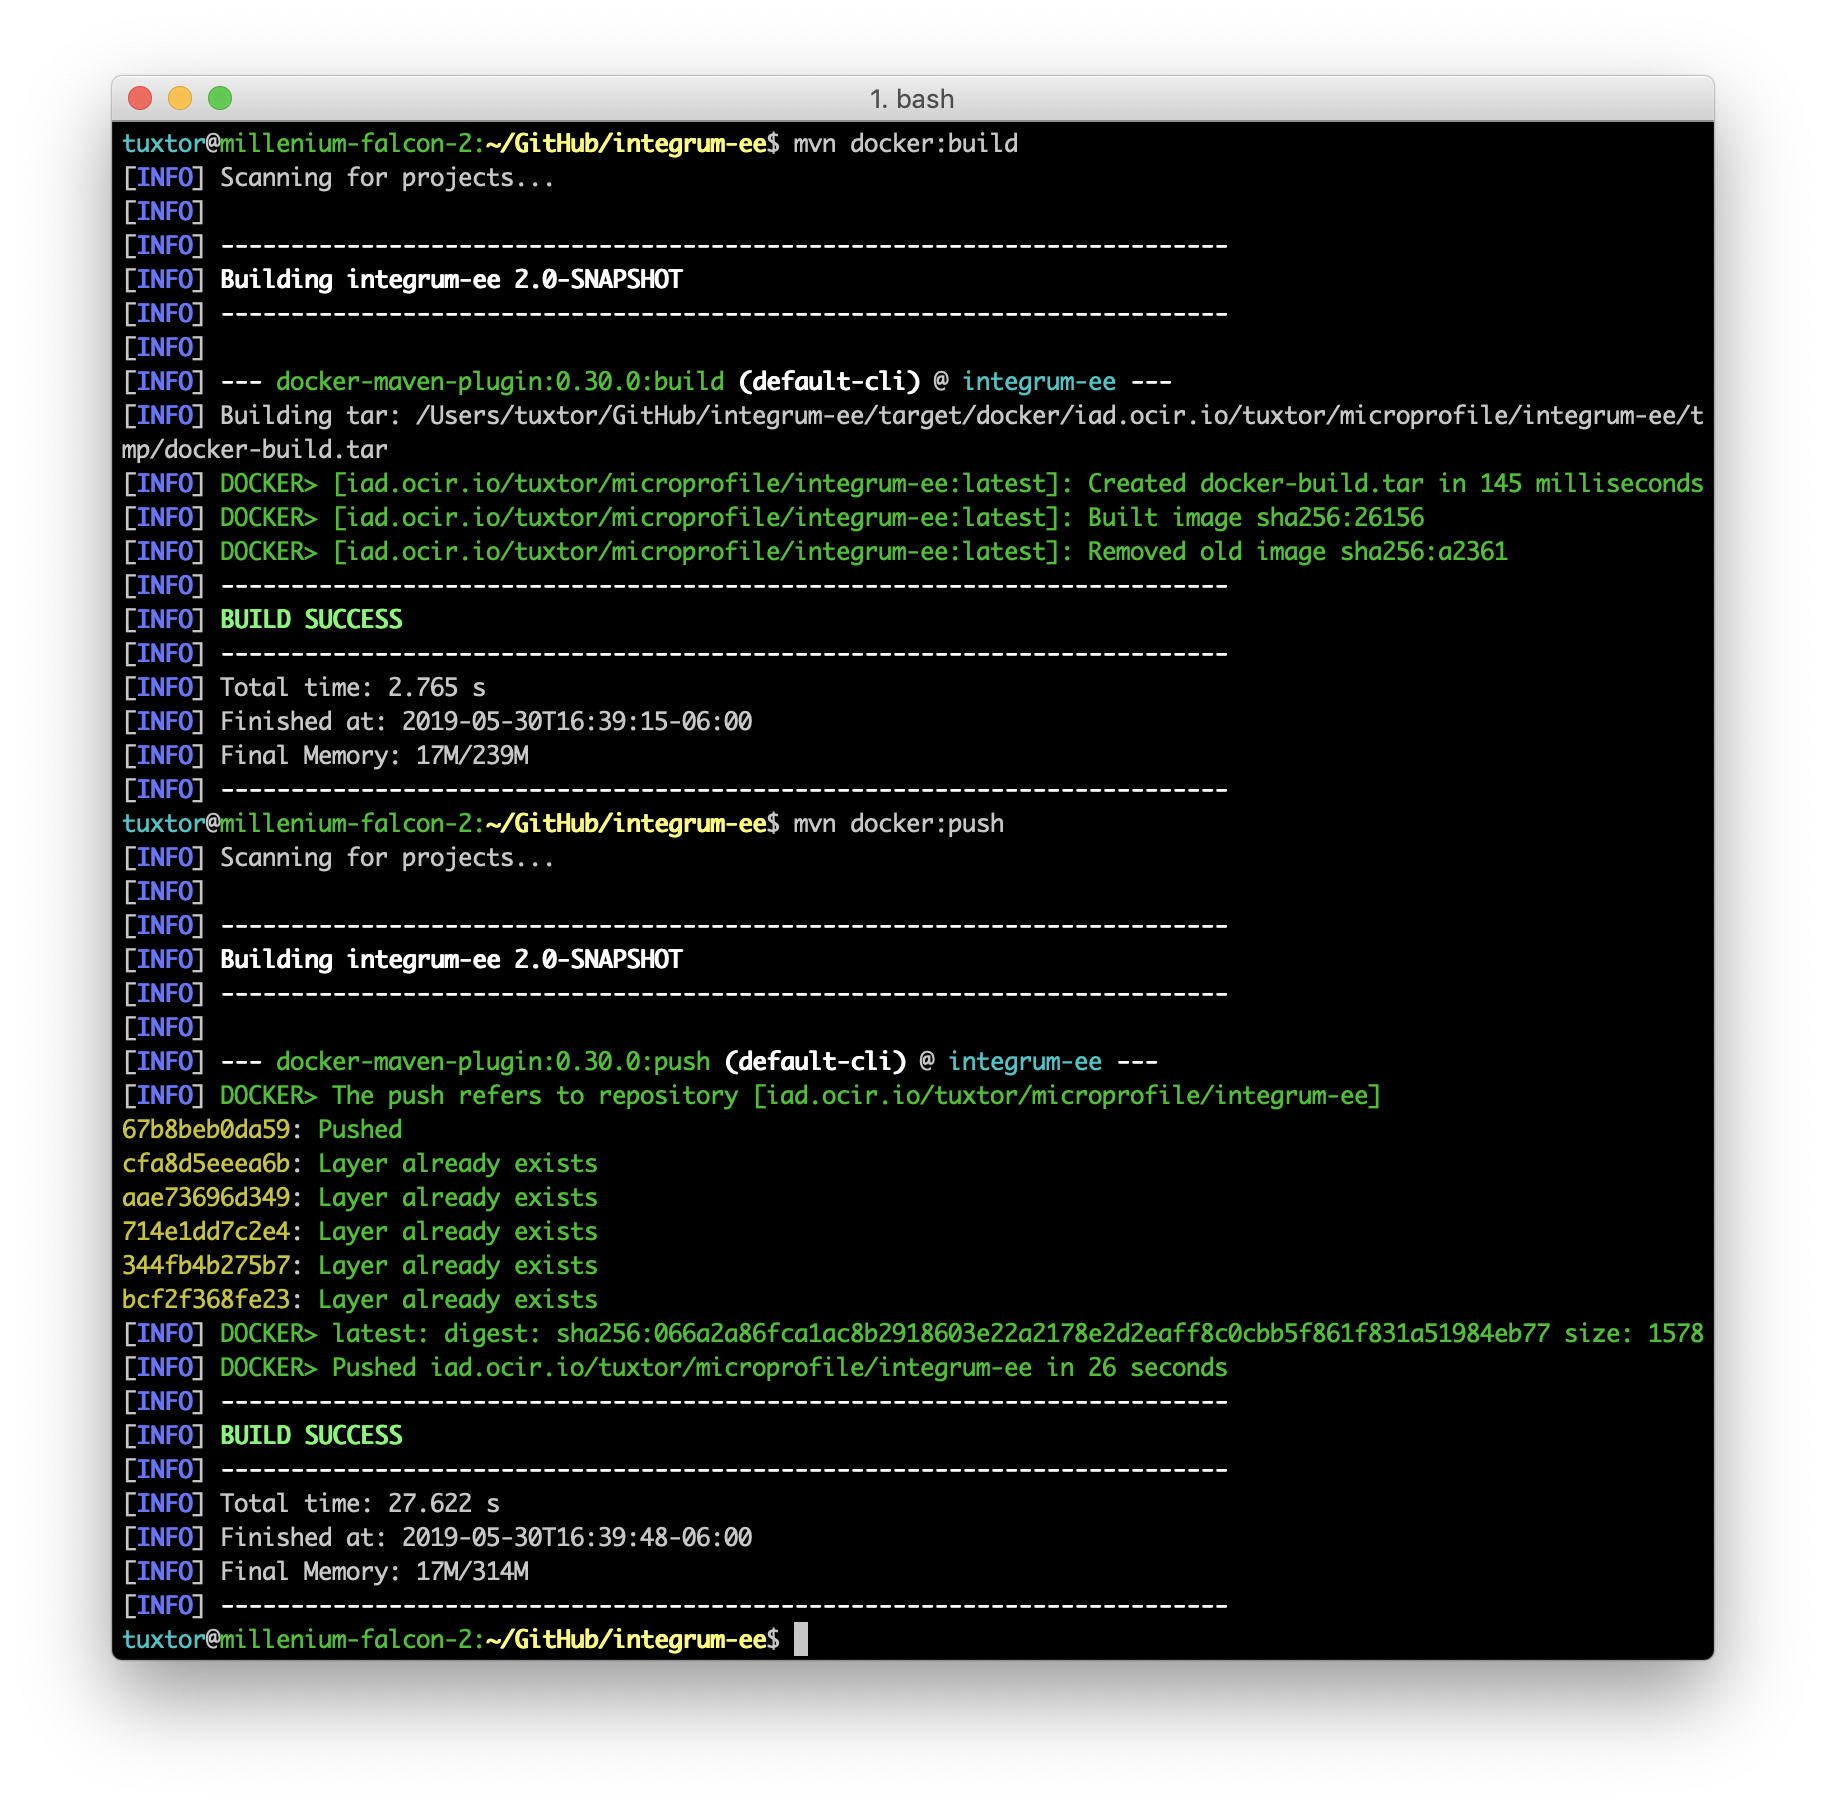
\includegraphics[width=\linewidth]{Images/oc3}
\end{figure}
\end{frame}

\begin{frame}{Oracle Cloud}

\begin{figure}
	\centering
	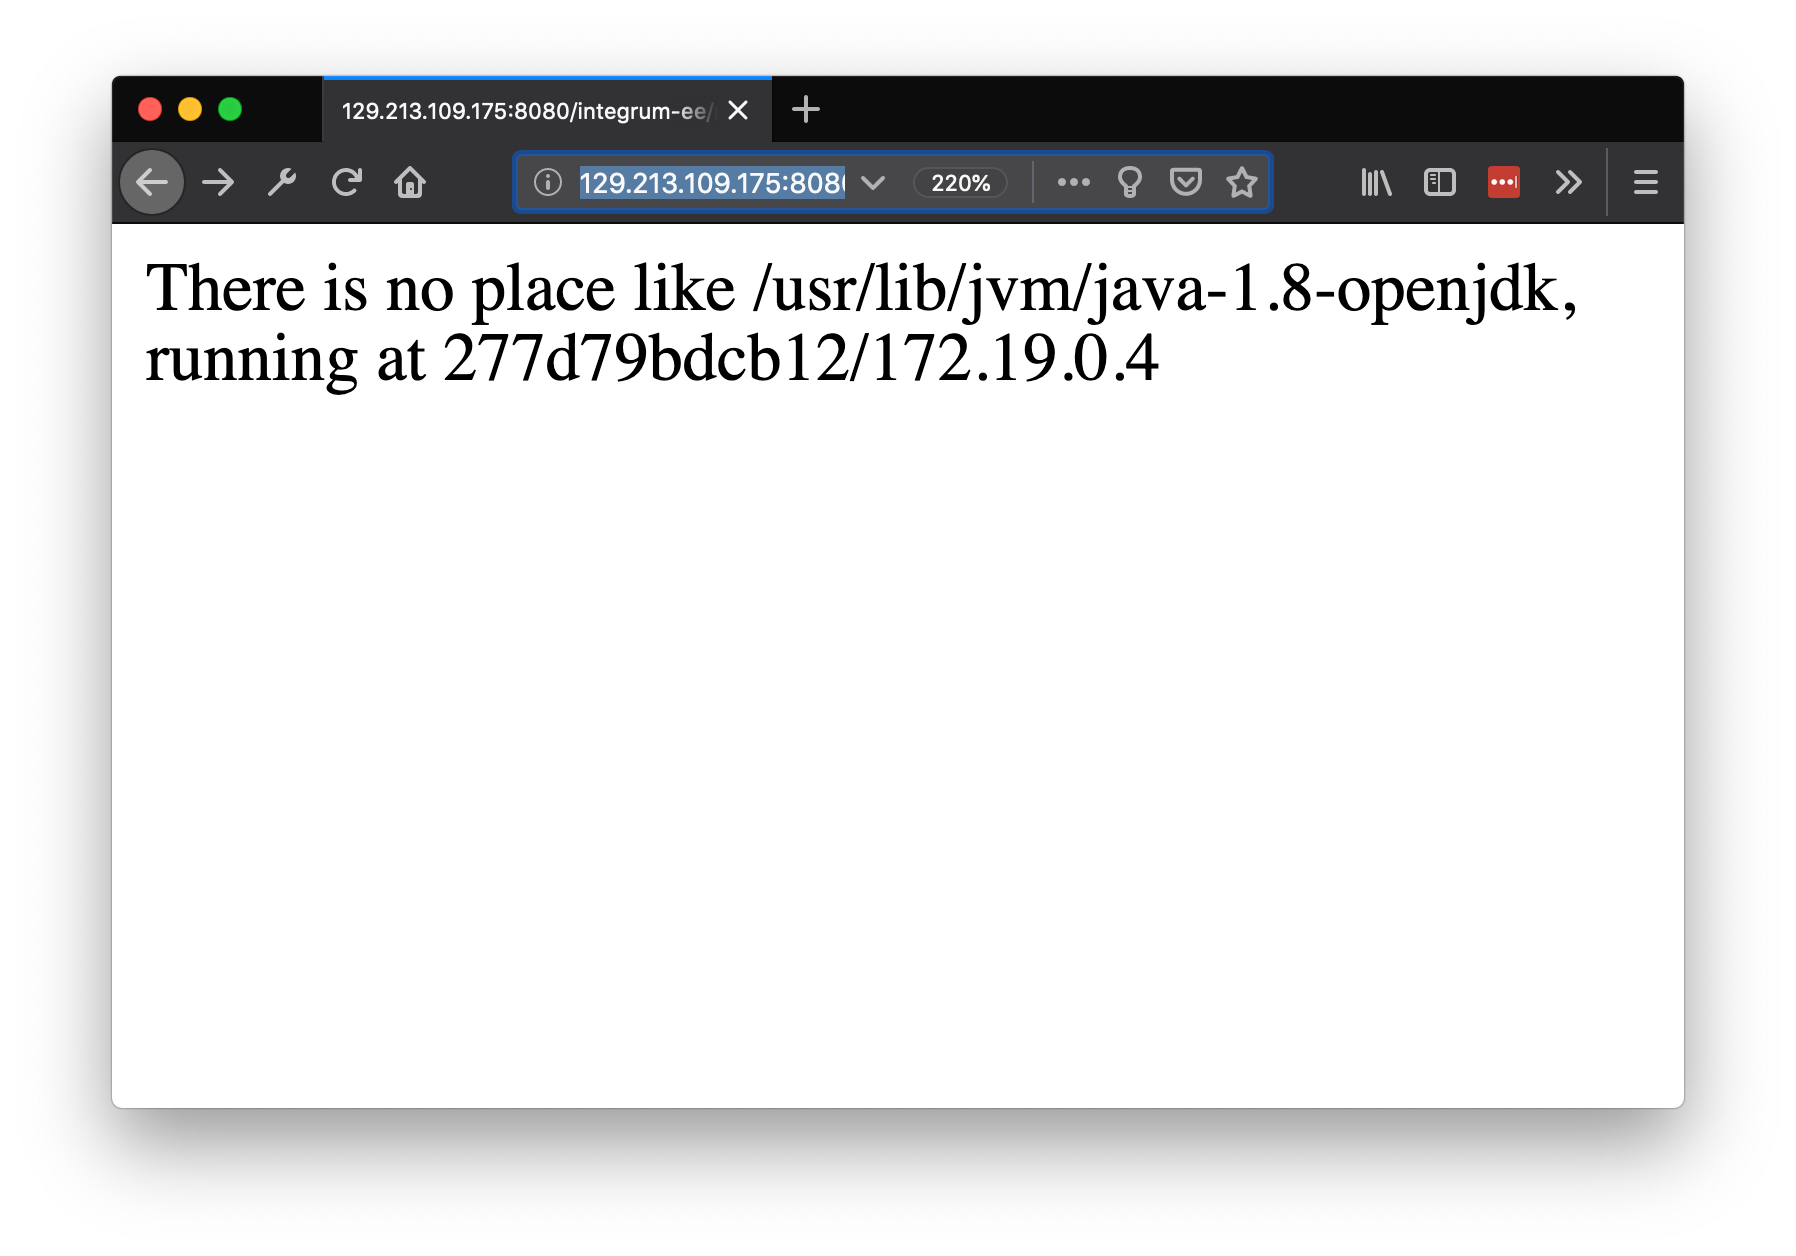
\includegraphics[width=\linewidth]{Images/oc4}
\end{figure}
\end{frame}

{
    \usebackgroundtemplate{
\includegraphics[width=\paperwidth]{Images/separador}}
    \setbeamercolor{normal text}{fg=white}
    \setbeamercolor{frametitle}{fg=red}
    \usebeamercolor[fg]{normal text}
    \section{Kotlin vs. Java}
}


\begin{frame}{Kotlin - Cosas más interesantes para mi}
\begin{columns}
	\begin{column}{0.5\textwidth}
		\begin{itemize}
			\item Static typing
			\item Java inter-op
			\item OO + FP
			\item Null safety
			\item Extension functions
			\item Operator overloading
			\item Data classes
			\item Functions as expressions
		\end{itemize}
	\end{column}
	\begin{column}{0.5\textwidth}  %%<--- here
		\begin{figure}
			\centering
			
\includegraphics[width=0.7\linewidth]{Images/kotlin}
		\end{figure}
	\end{column}
\end{columns}
\end{frame}

\begin{frame}{Kotlin - Datos interesantes}
\begin{columns}
\begin{column}{0.5\textwidth}
	\begin{itemize}
		\item Effective Java - Immutability, builder, singleton, override, final by default, variance by generics
		\item Elvis - Groovy
		\item Type inference - Scala
		\item Immutability - Scala
		\item Identifiers - Scala
		\item Null values management - Groovy
		\item Functions - Groovy
	\end{itemize}
\end{column}
\begin{column}{0.5\textwidth}  %%<--- here
	\begin{figure}
		\centering
		
\includegraphics[width=0.7\linewidth]{Images/kotlin}
	\end{figure}
\end{column}
\end{columns}
\end{frame}

\begin{frame}{Java - Muriendo desde 1995}
\begin{columns}
\begin{column}{0.5\textwidth}
\begin{itemize}
	\item Spring Boot, Micronaut, MicroProfile, GraalVM . . .
	\item Raw performance (Beam, Spark, Hadoop)
	\item Tooling - IDE, Maven, Drivers RDBMS
	\item JVM - (Twitter, Alibaba, Spotify, etc.)
	\item OpenJDK
\end{itemize}
\end{column}
\begin{column}{0.5\textwidth}  %%<--- here
\begin{figure}
	\centering
	
\includegraphics[width=0.4\linewidth]{Images/java}
\end{figure}
\end{column}
\end{columns}
\end{frame}

\begin{frame}{Kotlin}
\begin{columns}

	\begin{column}{0.5\textwidth}
		Ventajas
		\begin{itemize}
			\item Código conciso si se aprenden los nuevos bloques y expresiones
			\item Java inter-op
			\item Una oportunidad de Backend para desarrolladores Android
			\item Un nuevo abordaje "Full-stack"
		\end{itemize}
	\end{column}
	\begin{column}{0.5\textwidth}
		Desventajas
		\begin{itemize}
			\item IntelliJ IDEA Ultimate
			\item Curva de aprendizaje más pronunciada
			\item Compiler (time)
			\item Thread-managed vs Co-routines
			\item Amber, Loom, Valhalla, Panama (Java 18?)
		\end{itemize}
	\end{column}
\end{columns}
\end{frame}

\begin{frame}{Academik}
    \begin{columns}
        \begin{column}{0.7\textwidth}
            \begin{figure}
                \centering
                
\includegraphics[width=\linewidth]{Images/academik}
            \end{figure}
        \end{column}
        \begin{column}{0.3\textwidth}  %%<--- here
            \begin{figure}
                \centering
                
\includegraphics[width=\linewidth]{Images/qr}
            \end{figure}
        \end{column}
    \end{columns}
\end{frame}



\begin{frame}{Víctor Orozco}
\begin{columns}[T] % contents are top vertically aligned

	\begin{column}[T]{4cm} % alternative top-align that's better for graphics
		\begin{figure}
			\centering
			
\includegraphics[width=\linewidth]{Images/logos}
		\end{figure}
	\end{column}
	\begin{column}[T]{6cm} % each column can also be its own environment
		\begin{itemize}
			\item vorozco@nabenik.com
			\item \href{https://twitter.com/tuxtor}{@tuxtor}
			\item \href{http://www.nabenik.com}{https://vorozco.com}
		\end{itemize}
	\begin{center}
		
\includegraphics[width=0.1\linewidth]{Images/cclogo}
		\\
		This work is licensed under a Creative Commons Attribution-ShareAlike 3.0.
	\end{center}
	\end{column}
\end{columns}
\end{frame}


\end{document}

s